\documentclass[11pt]{article}
\usepackage{geometry}                % See geometry.pdf to learn the layout options. There are lots.
\geometry{letterpaper}                   % ... or a4paper or a5paper or ... 
%\geometry{landscape}                % Activate for for rotated page geometry
%\usepackage[parfill]{parskip}    % Activate to begin paragraphs with an empty line rather than an indent
\usepackage{graphicx}
\usepackage{amssymb,amsmath}
\usepackage{epstopdf}
\usepackage{pgf}
\usepackage{pgfpages}
\usepackage{tikz}
\usetikzlibrary{arrows,backgrounds}
\usepgflibrary{shapes}
\DeclareGraphicsRule{.tif}{png}{.png}{`convert #1 `dirname #1`/`basename #1 .tif`.png}
\pagestyle{empty}


\begin{document}

  \begin{center}
     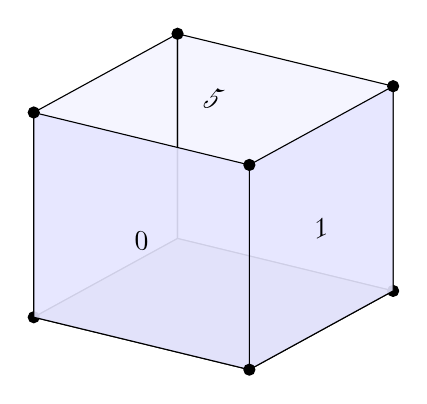
\begin{tikzpicture}[join=round] % Hexahedron Faces
         \filldraw[fill=blue!10,fill opacity=0.4](-2.282,2.433)--(-2.282,-.167)--(-.456,.833)--(-.456,3.433)--cycle;
         \filldraw[fill=blue!10,fill opacity=0.4](-.456,3.433)--(-.456,.833)--(2.282,.167)--(2.282,2.767)--cycle;
         \filldraw[fill=black!20](2.282,.167)--(-.456,.833)--(-2.282,-.167)--(.456,-.833)--cycle;
         \filldraw(-.456,3.433) circle (2pt);
         \filldraw(2.282,.167) circle (2pt);
         \filldraw[fill=blue!10,fill opacity=0.9](2.282,2.767)--(2.282,.167)--(.456,-.833)--(.456,1.767)--cycle;
         \filldraw(-2.282,-.167) circle (2pt);
         \filldraw[fill=blue!10,fill opacity=0.9](.456,1.767)--(.456,-.833)--(-2.282,-.167)--(-2.282,2.433)--cycle;
         \filldraw(2.282,2.767) circle (2pt);
         \filldraw(-2.282,2.433) circle (2pt);
         \filldraw(.456,-.833) circle (2pt);
         \filldraw(.456,1.767) circle (2pt);
         \fill[black]
                (0,2.6) node [xslant=.8,yslant=-.2] {5}
                (1.369,.967) node [yslant=0.5] {1}
                (-.913,.8) node [yslant=-.2] {0};
      \end{tikzpicture}
     \hspace{1cm}
     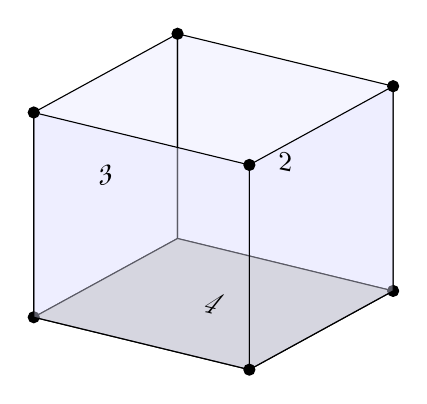
\begin{tikzpicture}[join=round] % Hexahedron Faces
         \filldraw[fill=blue!10,fill opacity=0.4](-2.282,2.433)--(-2.282,-.167)--(-.456,.833)--(-.456,3.433)--cycle;
         \filldraw[fill=blue!10,fill opacity=0.4](-.456,3.433)--(-.456,.833)--(2.282,.167)--(2.282,2.767)--cycle;
         \filldraw[fill=black!20](2.282,.167)--(-.456,.833)--(-2.282,-.167)--(.456,-.833)--cycle;
         \filldraw(-.456,3.433) circle (2pt);
         \filldraw(2.282,.167) circle (2pt);
         \filldraw[fill=blue!10,fill opacity=0.4](2.282,2.767)--(2.282,.167)--(.456,-.833)--(.456,1.767)--cycle;
         \filldraw(-2.282,-.167) circle (2pt);
         \filldraw[fill=blue!10,fill opacity=0.4](.456,1.767)--(.456,-.833)--(-2.282,-.167)--(-2.282,2.433)--cycle;
         \filldraw(2.282,2.767) circle (2pt);
         \filldraw(-2.282,2.433) circle (2pt);
         \filldraw(.456,-.833) circle (2pt);
         \filldraw(.456,1.767) circle (2pt);
         \fill[black]
                (0,0) node [xslant=0.8,yslant=-.2] {4}
                (-1.369,1.633) node [yslant=0.5] {3}
                (.913,1.8) node [yslant=-.2] {2};
      \end{tikzpicture}
  \end{center}
\end{document}  
